\documentclass[10pt,a4paper]{article}

% -----------------------------------------------------------------------------
% MATHS MANTHAN | Class 10 Areas Related to Circles Handbook | 2026--27
% Self-contained publication-quality master formula & concept handbook.
% Strictly compliant with the rationalized CBSE Class 10 curriculum.
% Exactly 14 Pages with zero overfull boxes or page overflow.
% -----------------------------------------------------------------------------

\usepackage[a4paper,top=12mm,bottom=15mm,left=15mm,right=15mm,footskip=8mm]{geometry}
\usepackage[T1]{fontenc}
\usepackage{lmodern}
\usepackage{microtype}
\usepackage{amsmath,amssymb}
\usepackage[table]{xcolor}
\usepackage{array,tabularx,booktabs}
\usepackage{graphicx}
\usepackage{eso-pic}
\usepackage{tikz}
\usetikzlibrary{calc,positioning,arrows.meta,shapes.geometric,patterns}
\usepackage[most]{tcolorbox}
\usepackage{enumitem}
\usepackage{fancyhdr}
\usepackage{lastpage}
\usepackage[hidelinks]{hyperref}
\usepackage{url}

% Compatibility fix for modern LaTeX/MiKTeX: colortbl + tabularx p-column alignment
\makeatletter
\let\insert@pcolumn\insert@column
\makeatother

% ============================================================================
% BRAND COLOR PALETTE — MATCHED TO THE MATHS MANTHAN STANDARD
% Primary navy: #001F49 | Brand gold: #D19029
% ============================================================================
\definecolor{primary}{RGB}{0,31,73}
\definecolor{brandnavy}{RGB}{0,31,73}
\definecolor{accent}{RGB}{209,144,41}
\definecolor{brandgold}{RGB}{209,144,41}
\definecolor{secondary}{RGB}{75,85,99}
\definecolor{lightgray}{RGB}{246,248,250}
\definecolor{accentlight}{RGB}{254,250,242}
\definecolor{primarylight}{RGB}{240,244,250}

\colorlet{navy}{primary}
\colorlet{blue}{primary!82!black}
\colorlet{gold}{accent}
\colorlet{goldpale}{accentlight}
\colorlet{bluepale}{primarylight}
\colorlet{ink}{secondary}
\colorlet{muted}{secondary}
\colorlet{linegray}{primary!25}
\colorlet{reddeep}{primary}
\colorlet{redpale}{lightgray}
\colorlet{green}{primary}
\colorlet{greenpale}{primarylight}

% Automatic low-opacity logo watermark on every page
\IfFileExists{mathsmanthan logo.png}{%
  \AddToShipoutPictureBG{%
    \begin{tikzpicture}[remember picture,overlay]
      \node[opacity=0.065] at (current page.center) {%
        \includegraphics[width=0.55\paperwidth,keepaspectratio]{mathsmanthan logo.png}%
      };
    \end{tikzpicture}%
  }%
}{}

\hypersetup{
  pdftitle={Class 10 Areas Related to Circles | Maths Manthan Handbook},
  pdfauthor={Maths Manthan Tuition Classes},
  pdfsubject={CBSE Class 10 Mathematics, Academic Year 2026--27},
  pdfkeywords={Areas Related to Circles, Class 10, CBSE, Mensuration, Sector, Segment, Maths Manthan, Formula Handbook}
}

\setlength{\parindent}{0pt}
\setlength{\parskip}{2pt}
\renewcommand{\arraystretch}{1.15}
\setlist[itemize]{leftmargin=4.5mm,itemsep=1pt,topsep=1pt,parsep=0pt}
\setlist[enumerate]{leftmargin=5.5mm,itemsep=1pt,topsep=1pt,parsep=0pt}
\setlength{\tabcolsep}{4.5pt}
\emergencystretch=2em
\hfuzz=1pt

% ============================================================================
% HEADER / FOOTER
% ============================================================================
\newcommand{\TuitionName}{{\color{primary}MATHS} {\color{accent}MANTHAN}}
\newcommand{\TuitionSub}{{\color{primary}\textbullet\ \ \text{TUITION CLASSES}\ \ \textbullet}}
\newcommand{\ContactInfo}{e-mail: contact@mathsmanthan.co.in \quad$\vert$\quad Helpline: +91-8171546558}
\newcommand{\HandbookFooterTitle}{Class 10 Areas Related to Circles Handbook}

\pagestyle{fancy}
\fancyhf{}
\renewcommand{\headrulewidth}{0pt}
\renewcommand{\footrulewidth}{0.6pt}
\renewcommand{\footrule}{\hbox to\headwidth{\color{primary!30}\leaders\hrule height 0.6pt\hfill}}
\fancyfoot[L]{\footnotesize\href{https://mathsmanthan.co.in}{\textcolor{secondary}{\TuitionName\ $\vert$\ \HandbookFooterTitle}}}
\fancyfoot[R]{\footnotesize\textbf{\color{primary}Page \thepage\ of \pageref{LastPage}}\quad\textcolor{accent}{\textbf{Academic Year 2026--27}}}

\fancypagestyle{plain}{%
  \fancyhf{}
  \fancyfoot[L]{\footnotesize\href{https://mathsmanthan.co.in}{\textcolor{secondary}{\TuitionName\ $\vert$\ \HandbookFooterTitle}}}
  \fancyfoot[R]{\footnotesize\textbf{\color{primary}Page \thepage\ of \pageref{LastPage}}\quad\textcolor{accent}{\textbf{Academic Year 2026--27}}}
  \renewcommand{\headrulewidth}{0pt}
  \renewcommand{\footrulewidth}{0.6pt}
  \renewcommand{\footrule}{\hbox to\headwidth{\color{primary!30}\leaders\hrule height 0.6pt\hfill}}
}

% Reusable design components
\newcommand{\BrandMark}{%
  \IfFileExists{mathsmanthan logo.png}{%
    \includegraphics[width=22mm,height=22mm,keepaspectratio]{mathsmanthan logo.png}%
  }{%
    
\begin{tikzpicture}[baseline=-0.6ex]
      \fill[navy,rounded corners=2.2pt] (0,0) rectangle (1.45,1.05);
      \draw[gold,line width=1.2pt] (0.15,0.15)--(1.30,0.15);
      \node[text=white,font=\sffamily\bfseries\Large] at (0.725,0.59) {MM};
    \end{tikzpicture}%
  }%
}

\newcommand{\chapterbanner}[4]{%
  \begin{tcolorbox}[enhanced,colback=bluepale,colframe=bluepale,boxrule=0pt,arc=2mm,
    left=3.5mm,right=3.5mm,top=1.8mm,bottom=1.8mm]
    {\footnotesize\bfseries\color{gold}CHAPTER #1\hfill\color{blue}#4}\par\vspace{0.4mm}
    {\Large\bfseries\color{navy}#2}\par
    {\small\color{muted}#3}
  \end{tcolorbox}\vspace{0.8mm}
}

\newcommand{\subhead}[1]{%
  \vspace{1mm}{\large\bfseries\color{navy}#1}\par\vspace{0.3mm}
  {\color{gold}\rule{14mm}{1.2pt}}\par\vspace{0.8mm}
}

\newtcolorbox{formulaBox}[1][]{enhanced,breakable,colback=goldpale,colframe=gold!65!black,
  boxrule=0.5pt,arc=1.5mm,left=2.8mm,right=2.8mm,top=1.8mm,bottom=1.8mm,
  before skip=2pt,after skip=3pt,#1}
\newtcolorbox{conceptBox}[1][]{enhanced,breakable,colback=bluepale,colframe=blue!25,
  boxrule=0.4pt,arc=1.5mm,left=2.8mm,right=2.8mm,top=1.8mm,bottom=1.8mm,
  before skip=2pt,after skip=3pt,#1}
\newtcolorbox{warningBox}[1][]{enhanced,breakable,colback=redpale,colframe=reddeep!45,
  boxrule=0.45pt,arc=1.5mm,left=2.8mm,right=2.8mm,top=1.8mm,bottom=1.8mm,
  before skip=2pt,after skip=3pt,#1}
\newtcolorbox{successBox}[1][]{enhanced,breakable,colback=greenpale,colframe=green!35,
  boxrule=0.45pt,arc=1.5mm,left=2.8mm,right=2.8mm,top=1.8mm,bottom=1.8mm,
  before skip=2pt,after skip=3pt,#1}

\newcommand{\CoreTag}{\tcbox[colback=greenpale,colframe=green!40,boxrule=.3pt,arc=1mm,left=1.5mm,right=1.5mm,top=.5mm,bottom=.5mm]{\scriptsize\bfseries\color{green}CORE SYLLABUS}}
\newcommand{\ExamTag}{\tcbox[colback=bluepale,colframe=blue!25,boxrule=.3pt,arc=1mm,left=1.5mm,right=1.5mm,top=.5mm,bottom=.5mm]{\scriptsize\bfseries\color{blue}EXAM STRATEGY}}
\newcommand{\TrapTag}{\tcbox[colback=redpale,colframe=reddeep!40,boxrule=.3pt,arc=1mm,left=1.5mm,right=1.5mm,top=.5mm,bottom=.5mm]{\scriptsize\bfseries\color{reddeep}TRAP ALERT}}
\newcommand{\ReferenceTag}{\tcbox[colback=bluepale,colframe=blue!25,boxrule=.3pt,arc=1mm,left=1.5mm,right=1.5mm,top=.5mm,bottom=.5mm]{\scriptsize\bfseries\color{blue}QUICK REFERENCE}}

\begin{document}

% =============================================================================
% PAGE 1: INSTITUTIONAL COVER PAGE
% =============================================================================
\thispagestyle{fancy}
\vspace*{0mm}
\noindent
\makebox[0pt][l]{%
  \raisebox{-0.80cm}[0pt][0pt]{%
    \href{https://mathsmanthan.co.in}{\BrandMark}%
  }%
}%
\parbox{\textwidth}{%
  \centering
  \href{https://mathsmanthan.co.in}{%
    {\fontsize{23pt}{23pt}\selectfont\bfseries \TuitionName}\\[3pt]
    {\footnotesize\bfseries \TuitionSub}%
  }\\[2pt]
  {\scriptsize\color{secondary} \ContactInfo}
}

\vspace{4pt}
\noindent{\color{primary}\rule{0.72\textwidth}{1.5pt}}\hfill{\color{accent}\rule{0.26\textwidth}{1.5pt}}

\vspace{3mm}
\begin{center}
  {\large\bfseries\color{muted}CBSE CLASS 10 \;$\vert$\; MATHEMATICS}\\[3mm]
  {\fontsize{26}{30}\selectfont\bfseries\color{navy}AREAS RELATED TO CIRCLES}\\[2mm]
  {\Large\color{blue}Master Concept, Formula \& Visual Problem-Solving Handbook}\\[2mm]
  {\large\color{gold}\bfseries Academic Year 2026--27}
\end{center}

\vspace{2.5mm}

\begin{tikzpicture}
  \fill[navy,rounded corners=3mm] (0,0) rectangle (\textwidth,2.8);
  \draw[gold,line width=2pt] (0.35,0.35)--(0.35,2.45);
  \node[anchor=west,text=white,font=\bfseries\Large] at (0.7,2.2) {See the region. Dissect the geometry.};
  \node[anchor=west,text=white,font=\Large] at (0.7,1.7) {Subtract with absolute precision.};
  \node[anchor=west,text=white,font=\small] at (0.7,1.1) {Sectors \;$\vert$\; Segments \;$\vert$\; Annulus \;$\vert$\; Combinations \;$\vert$\; Board Traps};
  \node[anchor=west,text=white!75,font=\footnotesize] at (0.7,0.55) {A student-first Maths Manthan conceptual and visual revision resource};
  \foreach \x/\r in {14.7/0.85,14.7/0.56,14.7/0.28} {\draw[gold!80,line width=1.1pt] (\x,1.4) circle (\r);}
  \fill[gold] (14.7,1.4) circle (0.08);
\end{tikzpicture}

\vspace{3mm}
\begin{minipage}[t]{0.48\textwidth}
  \begin{conceptBox}[title=What This Handbook Includes,fonttitle=\bfseries\color{navy}]
    \begin{itemize}
      \item Exact proofs of sector arc length and area formulas
      \item Universal $\triangle OAB$ trigonometric area derivation
      \item Inscribed/circumscribed polygons and combination figures
      \item Annulus, athletic track, and tethered grazing dynamics
      \item Clock face sweeps, automobile wipers, and brooches
      \item Master formula matrices and board audit protocols
    \end{itemize}
  \end{conceptBox}
\end{minipage}\hfill
\begin{minipage}[t]{0.48\textwidth}
  \begin{formulaBox}[title=Pedagogical Strategy: Foundations First,fonttitle=\bfseries\color{navy}]
    \raggedright Never blindly memorize formulas. Every sector is simply an angular fraction $\left(\frac{\theta}{360^\circ}\right)$ of a complete circle. Every segment is an elementary difference of two known shapes:
    $$\mathbf{\text{Segment} = \text{Sector } OAB - \triangle OAB}$$
    Always factor out common algebraic terms ($\pi r^2$, $r^2$) before evaluating numbers!
  \end{formulaBox}
\end{minipage}

\vspace{1.5mm}
\begin{warningBox}[title=CBSE 2026--27 Curriculum Verification \& Rationalized Scope,fonttitle=\bfseries\color{navy}]
  \textbf{Official Scope (Prescribed \& Tested):} Areas of sectors and segments of a circle (minor and major); length of corresponding arc; perimeter of a sector; area of combinations of plane figures involving circles, quadrants, semicircles, triangles, rectangles, and regular polygons. Central angles $\theta \in \{30^\circ, 45^\circ, 60^\circ, 90^\circ, 120^\circ\}$ are strictly in scope.\\
  \textbf{Excluded / Non-Examinable:} Calculus/integration area derivations; frustum of a cone cross-sections (shifted to Ch 12); geometric proofs of triangle similarity area ratios (deleted from Ch 6).
\end{warningBox}

\vfill
\begin{center}
  {\small\bfseries\color{navy}Maths Manthan Tuition Classes}\\
  {\footnotesize\color{muted}contact@mathsmanthan.co.in \quad$\vert$\quad +91-8171546558}\\
  {\footnotesize\url{https://mathsmanthan.co.in}}\\[1.5mm]
  {\scriptsize\color{muted}Prepared for learning and conceptual mastery \;--\; Strictly aligned with CBSE Class 10 Syllabus 2026--27.}
\end{center}

\newpage

% =============================================================================
% PAGE 2: MODULE 1 — CIRCLE ANATOMY, PI & WHEEL KINEMATICS
% =============================================================================
\thispagestyle{fancy}
\vspace*{0mm}

\chapterbanner{11}{AREAS RELATED TO CIRCLES}{Module 1 $\vert$ Foundations: Anatomy, The Geometry of $\pi$ \& Wheel Kinematics}{\CoreTag}

\subhead{1.1 Anatomy of a Circle and Prerequisite Metrics}

A \textbf{circle} is the locus of all points in a plane situated at a fixed distance (radius $r$) from a fixed center $O$.

\begin{minipage}[c]{0.44\textwidth}
\centering
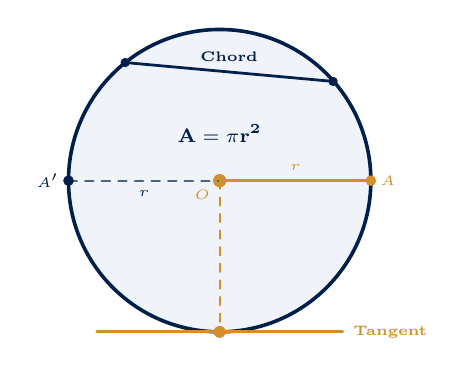
\begin{tikzpicture}[scale=1.2, line cap=round, line join=round]
  \draw[primary!20, fill=primarylight, line width=0.9pt] (0,0) circle (1.6cm);
  \draw[primary, line width=1.3pt] (0,0) circle (1.6cm);

  \fill[accent] (0,0) circle (2pt) node[below left, font=\tiny\bfseries\color{navy}]{$O$};
  \draw[accent, line width=1.2pt] (0,0) -- (1.6,0);
  \fill[accent] (1.6,0) circle (1.6pt) node[right, font=\tiny\bfseries\color{navy}]{$A$};
  \node[font=\tiny\bfseries\color{accent}, above] at (0.8,0) {$r$};

  \draw[dashed, primary!70, line width=0.8pt] (-1.6,0) -- (0,0);
  \fill[primary] (-1.6,0) circle (1.6pt) node[left, font=\tiny\bfseries\color{navy}]{$A'$};
  \node[font=\tiny\bfseries\color{primary}, below] at (-0.8,0) {$r$};

  \coordinate (C1) at (-1.0,1.25);
  \coordinate (C2) at (1.2,1.05);
  \draw[primary, line width=1pt] (C1) -- (C2) node[midway, above, font=\tiny\bfseries\color{navy}]{Chord};
  \fill[primary] (C1) circle (1.4pt);
  \fill[primary] (C2) circle (1.4pt);

  \coordinate (T) at (0,-1.6);
  \draw[accent, line width=1.1pt] (-1.3,-1.6) -- (1.3,-1.6) node[right, font=\tiny\bfseries\color{accent}]{Tangent};
  \fill[accent] (T) circle (1.8pt);
  \draw[dashed, accent, line width=0.7pt] (0,0) -- (0,-1.6);

  \node[font=\scriptsize\bfseries\color{navy}, align=center] at (0,0.5) {$\mathbf{A = \pi r^2}$};
\end{tikzpicture}
\end{minipage}\hfill
\begin{minipage}[c]{0.54\textwidth}
\begin{formulaBox}
  \textbf{Fundamental Metrics of a Circle of Radius $r$:}
  \begin{itemize}
    \item \textbf{Diameter ($d$):} $\mathbf{d = 2r \iff r = d/2}$
    \item \textbf{Circumference ($C$):} Perimeter of boundary:
      $$\mathbf{C = 2\pi r = \pi d}$$
    \item \textbf{Enclosed Area ($A$):} 2D region bounded by curve:
      $$\mathbf{A = \pi r^2 = \pi (d/2)^2 = \frac{1}{4}\pi d^2}$$
    \item \textbf{Semicircle ($180^\circ$):}
      $$\text{Area} = \mathbf{\frac{1}{2}\pi r^2}, \quad \text{Perimeter} = \mathbf{\pi r + 2r}$$
    \item \textbf{Quadrant ($90^\circ$):}
      $$\text{Area} = \mathbf{\frac{1}{4}\pi r^2}, \quad \text{Perimeter} = \mathbf{\frac{1}{2}\pi r + 2r}$$
  \end{itemize}
\end{formulaBox}
\end{minipage}

\vspace{0.8mm}
\subhead{1.2 The Geometric Constant $\pi$ (Pi): Concept and Conventions}

By definition, $\mathbf{\pi}$ is the ratio of the circumference of any circle to its diameter: $\pi = \frac{C}{2r}$.
$\pi$ is an \textbf{irrational number} ($\pi \approx 3.14159265\dots$). Aryabhata gave the approximation $\pi \approx \frac{62832}{20000} = 3.1416$.
\begin{itemize}
  \item \textbf{CBSE Rule:} Always use $\mathbf{\pi = \frac{22}{7}}$ unless explicitly instructed to take $\mathbf{\pi = 3.14}$.
\end{itemize}

\vspace{0.8mm}
\subhead{1.3 Linear Kinematics of a Rolling Wheel (Revolutions \& Distance)}

When a circular wheel of radius $r$ completes \textbf{one revolution} without slipping, the linear distance covered along the ground is exactly equal to its circumference:
$$\mathbf{\text{Distance in 1 revolution} = 2\pi r} \quad \implies \quad \mathbf{\text{Total Distance: } D = N \times 2\pi r \iff N = \frac{D}{2\pi r} = \frac{D}{\pi d}}$$

\begin{conceptBox}[title={Worked Archetype 1 $\vert$ Rotational Speed \& Number of Revolutions},fonttitle=\bfseries\color{navy}]
  \textbf{Problem:} The wheels of a car are of diameter $80\text{ cm}$ each. How many complete revolutions does each wheel make in $10\text{ minutes}$ when the car travels at $66\text{ km/h}$? (Take $\pi = \frac{22}{7}$)
  \par\vspace{0.6mm}\noindent
  \textbf{Step 1: Unify units:} $d = 80\text{ cm} \implies r = 40\text{ cm} = 0.4\text{ m}$. Speed $v = \frac{66 \times 1000\text{ m}}{60\text{ min}} = 1100\text{ m/min}$.\\
  \textbf{Step 2: Total distance in 10 minutes:} $D = 1100\text{ m/min} \times 10\text{ min} = 11{,}000\text{ m} = 1{,}100{,}000\text{ cm}$.\\
  \textbf{Step 3: Distance in 1 revolution:} $C = 2\pi r = 2 \times \frac{22}{7} \times 40 = \frac{1760}{7}\text{ cm}$.\\
  \textbf{Step 4: Revolutions:} $N = \frac{D}{C} = \frac{1{,}100{,}000 \times 7}{1760} = \mathbf{4375\text{ complete revolutions.}}$
\end{conceptBox}

\newpage

% =============================================================================
% PAGE 3: MODULE 2 — SECTORS OF A CIRCLE (ARC LENGTH & SECTOR AREA)
% =============================================================================
\thispagestyle{fancy}
\vspace*{0mm}

\chapterbanner{11}{AREAS RELATED TO CIRCLES}{Module 2 $\vert$ Sectors: Arc Length, Sector Area \& Perimeter}{\CoreTag}

\subhead{2.1 The Concept of a Circular Sector}

A \textbf{sector} is the portion of a circular disc enclosed by two radii ($OA$ and $OB$) and the arc ($AB$) subtending a central angle $\theta$ at the center $O$.
\begin{itemize}
  \item \textbf{Minor Sector:} The sector subtending central angle $\theta < 180^\circ$.
  \item \textbf{Major Sector:} The remainder of the circular disc, subtending central angle $(360^\circ - \theta)$.
\end{itemize}

\begin{minipage}[c]{0.43\textwidth}
\centering
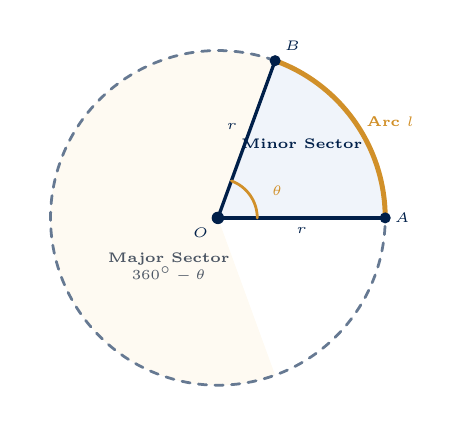
\begin{tikzpicture}[scale=1.25, line cap=round, line join=round]
  \fill[accentlight] (0,0) -- (1.7,0) arc (0:290:1.7cm) -- cycle;
  \fill[primarylight] (0,0) -- (1.7,0) arc (0:70:1.7cm) -- cycle;

  \draw[primary, line width=1.2pt] (0,0) -- (1.7,0);
  \draw[primary, line width=1.2pt] (0,0) -- ({1.7*cos(70)},{1.7*sin(70)});
  \draw[accent, line width=1.8pt] (1.7,0) arc (0:70:1.7cm) node[midway, right, font=\tiny\bfseries\color{accent}]{Arc $l$};
  \draw[primary!60, line width=1pt, dashed] ({1.7*cos(70)},{1.7*sin(70)}) arc (70:360:1.7cm);

  \fill[primary] (0,0) circle (1.8pt) node[below left, font=\tiny\bfseries]{$O$};
  \fill[primary] (1.7,0) circle (1.6pt) node[right, font=\tiny\bfseries]{$A$};
  \fill[primary] ({1.7*cos(70)},{1.7*sin(70)}) circle (1.6pt) node[above right, font=\tiny\bfseries]{$B$};

  \draw[accent, line width=1pt] (0.4,0) arc (0:70:0.4cm);
  \node[font=\tiny\bfseries\color{accent}] at (0.6,0.28) {$\theta$};

  \node[font=\tiny\bfseries\color{navy}, below] at (0.85,0) {$r$};
  \node[font=\tiny\bfseries\color{navy}, above left] at ({0.85*cos(70)},{0.85*sin(70)}) {$r$};

  \node[font=\tiny\bfseries\color{navy}, align=center] at (0.85,0.75) {Minor Sector};
  \node[font=\tiny\bfseries\color{secondary}, align=center] at (-0.5,-0.5) {Major Sector\\$360^\circ - \theta$};
\end{tikzpicture}
\end{minipage}\hfill
\begin{minipage}[c]{0.55\textwidth}
\begin{formulaBox}
  \textbf{Universal Sector Formulas (Angle $\theta$ in degrees):}
  \begin{itemize}
    \item \textbf{Length of Arc ($l$):}
      $$\mathbf{l = \frac{\theta}{360^\circ} \times 2\pi r = \frac{\theta}{180^\circ} \times \pi r}$$
    \item \textbf{Area of Sector ($A$):}
      $$\mathbf{A = \frac{\theta}{360^\circ} \times \pi r^2}$$
    \item \textbf{Relation Between Arc Length $l$ and Area $A$:}
      $$\mathbf{A = \frac{1}{2} \cdot l \cdot r} \quad \left(\text{Like } \frac{1}{2} \times \text{base} \times \text{height}\right)$$
    \item \textbf{Perimeter of Sector ($P$):}
      $$\mathbf{P = l + 2r = \frac{\theta}{360^\circ} \times 2\pi r + 2r}$$
    \item \textbf{Area of Major Sector:}
      $$\mathbf{A_{\text{major}} = \pi r^2 - A_{\text{minor}} = \frac{360^\circ - \theta}{360^\circ} \times \pi r^2}$$
  \end{itemize}
\end{formulaBox}
\end{minipage}

\vspace{0.8mm}
\subhead{2.2 The Fatal ``Sector Perimeter'' Board Trap}

\begin{warningBox}
  \textbf{\TrapTag\ Arc Length $\neq$ Perimeter of Sector!}
  In board exams, many students write $P = l$. An arc is an \textbf{open curve}. To form a closed sector, you \textbf{must add both bounding radii} $OA$ and $OB$:
  $$\mathbf{\text{Perimeter of Sector} = \text{Arc Length } (l) + 2 \times \text{Radius } (r) = l + 2r}$$
\end{warningBox}

\vspace{0.8mm}
\begin{conceptBox}[title={Worked Archetype 2 $\vert$ Arc Length, Sector Area, and Perimeter},fonttitle=\bfseries\color{navy}]
  \textbf{Problem:} In a circle of radius $21\text{ cm}$, an arc subtends an angle of $60^\circ$ at the centre. Find: (i) length of the arc, (ii) area of the sector formed by the arc, and (iii) perimeter of the sector. (Take $\pi = \frac{22}{7}$)
  \par\vspace{0.6mm}\noindent
  \textbf{Solution:} Given $r = 21\text{ cm}$, central angle $\theta = 60^\circ$.
  \begin{enumerate}
    \item \textbf{Length of the arc ($l$):}
      $l = \frac{60^\circ}{360^\circ} \times 2 \times \frac{22}{7} \times 21 = \frac{1}{6} \times 2 \times 22 \times 3 = \mathbf{22\text{ cm}}$.
    \item \textbf{Area of the sector ($A$):}
      $A = \frac{60^\circ}{360^\circ} \times \frac{22}{7} \times 21 \times 21 = \frac{1}{6} \times 22 \times 3 \times 21 = 11 \times 21 = \mathbf{231\text{ cm}^2}$.\\
      \textit{Alternative Verification:} $A = \frac{1}{2} l r = \frac{1}{2} \times 22 \times 21 = \mathbf{231\text{ cm}^2}$.
    \item \textbf{Perimeter of the sector ($P$):}
      $P = l + 2r = 22 + 2(21) = 22 + 42 = \mathbf{64\text{ cm}}$.
  \end{enumerate}
\end{conceptBox}

\newpage

% =============================================================================
% PAGE 4: MODULE 3 — SEGMENTS OF A CIRCLE (MINOR & MAJOR SEGMENTS)
% =============================================================================
\thispagestyle{fancy}
\vspace*{0mm}

\chapterbanner{11}{AREAS RELATED TO CIRCLES}{Module 3 $\vert$ Segments of a Circle: Dissection, Area \& Formulas}{\CoreTag}

\subhead{3.1 The Geometric Definition of a Circular Segment}

A \textbf{segment} of a circle is the region bounded by a chord ($AB$) and the corresponding arc connecting its endpoints:
\begin{itemize}
  \item \textbf{Minor Segment:} Region bounded by chord $AB$ and minor arc $APB$.
  \item \textbf{Major Segment:} Region bounded by chord $AB$ and major arc $AQB$.
\end{itemize}

\begin{minipage}[c]{0.42\textwidth}
\centering
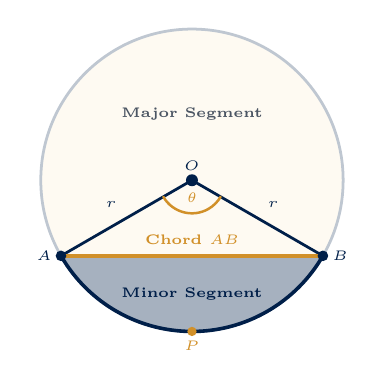
\begin{tikzpicture}[scale=1.2, line cap=round, line join=round]
  \draw[primary!25, fill=accentlight, line width=1pt] (0,0) circle (1.6cm);

  \coordinate (O) at (0,0);
  \coordinate (A) at ({1.6*cos(210)},{1.6*sin(210)});
  \coordinate (B) at ({1.6*cos(330)},{1.6*sin(330)});

  \fill[primary!35] (A) -- (B) arc (330:210:1.6cm) -- cycle;

  \draw[primary, line width=1pt] (O) -- (A) node[midway, above left, font=\tiny]{$r$};
  \draw[primary, line width=1pt] (O) -- (B) node[midway, above right, font=\tiny]{$r$};
  \draw[accent, line width=1.4pt] (A) -- (B) node[midway, above, font=\tiny\bfseries\color{accent}]{Chord $AB$};
  \draw[primary, line width=1.3pt] (A) arc (210:330:1.6cm);

  \fill[primary] (O) circle (1.8pt) node[above, font=\tiny\bfseries]{$O$};
  \fill[primary] (A) circle (1.6pt) node[left, font=\tiny\bfseries]{$A$};
  \fill[primary] (B) circle (1.6pt) node[right, font=\tiny\bfseries]{$B$};
  \coordinate (P) at ({1.6*cos(270)},{1.6*sin(270)});
  \fill[accent] (P) circle (1.4pt) node[below, font=\tiny\bfseries\color{accent}]{$P$};

  \draw[accent, line width=0.9pt] ({0.35*cos(210)},{0.35*sin(210)}) arc (210:330:0.35cm);
  \node[font=\tiny\bfseries\color{accent}] at (0,-0.18) {$\theta$};

  \node[font=\tiny\bfseries\color{navy}, align=center] at (0,-1.2) {Minor Segment};
  \node[font=\tiny\bfseries\color{secondary}, align=center] at (0,0.7) {Major Segment};
\end{tikzpicture}
\end{minipage}\hfill
\begin{minipage}[c]{0.56\textwidth}
\begin{formulaBox}
  \textbf{The Universal Segment Dissection Axiom:}
  $$\mathbf{A_{\text{minor}} = \text{Area}(\text{Sector } OAPB) - \text{Area}(\triangle OAB)}$$
  $$\mathbf{A_{\text{major}} = \text{Area of Circle} - A_{\text{minor}} = \pi r^2 - A_{\text{minor}}}$$
  \textbf{Universal Triangle Formula:}
  $$\mathbf{\text{Area}(\triangle OAB) = \frac{1}{2} r^2 \sin\theta}$$
  $$\mathbf{A_{\text{minor}} = r^2\left[\frac{\pi\theta}{360^\circ} - \frac{1}{2}\sin\theta\right]}$$
\end{formulaBox}
\end{minipage}

\vspace{0.8mm}
\subhead{3.2 Rigorous Derivation: $\text{Area}(\triangle OAB) = \frac{1}{2}r^2\sin\theta$}

\begin{minipage}[c]{0.56\textwidth}
Draw $OM \perp AB$. In isosceles triangle $\triangle OAB$ ($OA = OB = r$):
\begin{enumerate}
  \item Altitude $OM$ bisects chord $AB$ and vertex angle $\angle AOB = \theta$:
    $$\angle AOM = \angle BOM = \frac{\theta}{2}$$
  \item In right $\triangle OAM$:
    $$AM = r\sin(\theta/2) \implies AB = 2r\sin(\theta/2)$$
    $$OM = r\cos(\theta/2)$$
  \item Triangle Area:
    $$\text{Area} = \frac{1}{2} \cdot AB \cdot OM = \frac{1}{2}[2r\sin(\theta/2)][r\cos(\theta/2)]$$
    $$\text{Area} = r^2 \sin(\theta/2)\cos(\theta/2) = \mathbf{\frac{1}{2}r^2\sin\theta}$$
\end{enumerate}
\end{minipage}\hfill
\begin{minipage}[c]{0.42\textwidth}
\centering
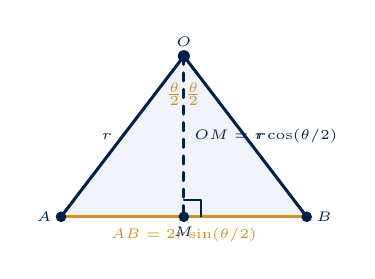
\begin{tikzpicture}[scale=1.2, line cap=round, line join=round]
  \coordinate (O) at (0,1.7);
  \coordinate (A) at (-1.3,0);
  \coordinate (B) at (1.3,0);
  \coordinate (M) at (0,0);

  \fill[primarylight] (O) -- (A) -- (B) -- cycle;
  \draw[primary, line width=1.1pt] (O) -- (A) node[midway, left, font=\tiny]{$r$};
  \draw[primary, line width=1.1pt] (O) -- (B) node[midway, right, font=\tiny]{$r$};
  \draw[accent, line width=1.2pt] (A) -- (B) node[midway, below, font=\tiny\bfseries\color{accent}]{$AB = 2r\sin(\theta/2)$};
  \draw[dashed, reddeep, line width=1pt] (O) -- (M) node[midway, right, font=\tiny\bfseries\color{reddeep}]{$OM = r\cos(\theta/2)$};

  \draw[reddeep, line width=0.6pt] (0,0.18) -- (0.18,0.18) -- (0.18,0);

  \fill[primary] (O) circle (1.8pt) node[above, font=\tiny\bfseries]{$O$};
  \fill[primary] (A) circle (1.6pt) node[left, font=\tiny\bfseries]{$A$};
  \fill[primary] (B) circle (1.6pt) node[right, font=\tiny\bfseries]{$B$};
  \fill[reddeep] (M) circle (1.6pt) node[below, font=\tiny\bfseries\color{reddeep}]{$M$};
  \node[font=\tiny\bfseries\color{accent}] at (-0.1,1.3) {$\frac{\theta}{2}$};
  \node[font=\tiny\bfseries\color{accent}] at (0.1,1.3) {$\frac{\theta}{2}$};
\end{tikzpicture}
\end{minipage}

\newpage

% =============================================================================
% PAGE 5: MODULE 4 — MASTER ANGLE & TRIGONOMETRIC EVALUATION MATRIX
% =============================================================================
\thispagestyle{fancy}
\vspace*{0mm}

\chapterbanner{11}{AREAS RELATED TO CIRCLES}{Module 4 $\vert$ Master Angle Evaluation: $\theta \in \{60^\circ, 90^\circ, 120^\circ\}$}{\CoreTag}

\subhead{4.1 Exact Evaluation of $\triangle OAB$ Across Board-Mandated Angles}

The CBSE Class 10 examination focuses on three primary central angles for segment problems:

\begin{center}
\small
\begin{tabularx}{\textwidth}{c c c c >{\bfseries}l X}
\toprule
\rowcolor{bluepale}
$\theta$ & $\sin\theta$ & $\frac{\theta}{360^\circ}$ & $\triangle OAB$ Type & $\text{Area}(\triangle OAB)$ Formula & Visual Geometric Shortcut \\
\midrule
$\mathbf{60^\circ}$ & $\frac{\sqrt{3}}{2}$ & $\frac{1}{6}$ & Equilateral & $\mathbf{\frac{\sqrt{3}}{4}r^2}$ & Since $OA=OB$ and $\angle O=60^\circ$, all angles are $60^\circ$. \\
\midrule
$\mathbf{90^\circ}$ & $1$ & $\frac{1}{4}$ & Right-Isosceles & $\mathbf{\frac{1}{2}r^2}$ & Base $= r$, Perpendicular Altitude $= r \implies \frac{1}{2}r \cdot r$. \\
\midrule
$\mathbf{120^\circ}$ & $\frac{\sqrt{3}}{2}$ & $\frac{1}{3}$ & Obtuse Isosceles & $\mathbf{\frac{\sqrt{3}}{4}r^2}$ & Base $= r\sqrt{3}$, Altitude $= \frac{1}{2}r \implies \frac{1}{2}(r\sqrt{3})(\frac{1}{2}r)$. \\
\bottomrule
\end{tabularx}
\end{center}

\vspace{0.5mm}
\subhead{4.2 Geometric Visual Architectures for $60^\circ$, $90^\circ$, and $120^\circ$}

\begin{center}
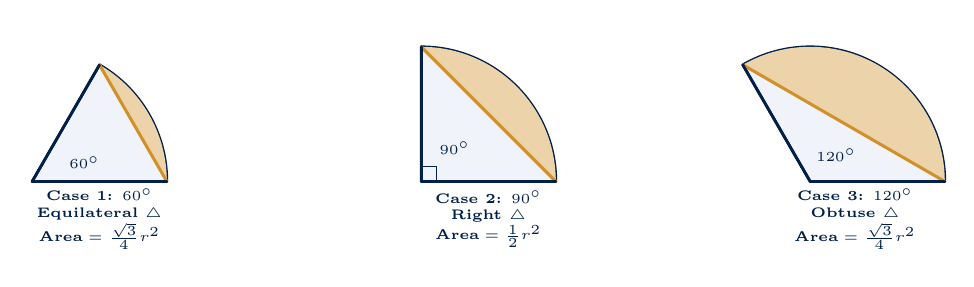
\begin{tikzpicture}[scale=0.95, line cap=round, line join=round]
  % 60 deg
  \begin{scope}[shift={(0,0)}]
    \draw[primary, fill=primarylight, line width=1pt] (0,0) -- (1.8,0) arc (0:60:1.8cm) -- cycle;
    \fill[accent!40] (1.8,0) -- ({1.8*cos(60)},{1.8*sin(60)}) arc (60:0:1.8cm) -- cycle;
    \draw[accent, line width=1.1pt] (1.8,0) -- ({1.8*cos(60)},{1.8*sin(60)});
    \draw[primary, line width=1pt] (0,0) -- (1.8,0);
    \draw[primary, line width=1pt] (0,0) -- ({1.8*cos(60)},{1.8*sin(60)});
    \node[font=\tiny\bfseries\color{navy}] at (0.7,0.25) {$60^\circ$};
    \node[font=\tiny\bfseries\color{navy}, align=center] at (0.9,-0.5) {\textbf{Case 1: $60^\circ$}\\Equilateral $\triangle$\\$\text{Area} = \frac{\sqrt{3}}{4}r^2$};
  \end{scope}

  % 90 deg
  \begin{scope}[shift={(5.2,0)}]
    \draw[primary, fill=primarylight, line width=1pt] (0,0) -- (1.8,0) arc (0:90:1.8cm) -- cycle;
    \fill[accent!40] (1.8,0) -- (0,1.8) arc (90:0:1.8cm) -- cycle;
    \draw[accent, line width=1.1pt] (1.8,0) -- (0,1.8);
    \draw[primary, line width=1pt] (0,0) -- (1.8,0);
    \draw[primary, line width=1pt] (0,0) -- (0,1.8);
    \draw[primary] (0,0.2) -- (0.2,0.2) -- (0.2,0);
    \node[font=\tiny\bfseries\color{navy}] at (0.45,0.45) {$90^\circ$};
    \node[font=\tiny\bfseries\color{navy}, align=center] at (0.9,-0.5) {\textbf{Case 2: $90^\circ$}\\Right $\triangle$\\$\text{Area} = \frac{1}{2}r^2$};
  \end{scope}

  % 120 deg
  \begin{scope}[shift={(10.4,0)}]
    \draw[primary, fill=primarylight, line width=1pt] (0,0) -- (1.8,0) arc (0:120:1.8cm) -- cycle;
    \fill[accent!40] (1.8,0) -- ({1.8*cos(120)},{1.8*sin(120)}) arc (120:0:1.8cm) -- cycle;
    \draw[accent, line width=1.1pt] (1.8,0) -- ({1.8*cos(120)},{1.8*sin(120)});
    \draw[primary, line width=1pt] (0,0) -- (1.8,0);
    \draw[primary, line width=1pt] (0,0) -- ({1.8*cos(120)},{1.8*sin(120)});
    \node[font=\tiny\bfseries\color{navy}] at (0.35,0.35) {$120^\circ$};
    \node[font=\tiny\bfseries\color{navy}, align=center] at (0.6,-0.5) {\textbf{Case 3: $120^\circ$}\\Obtuse $\triangle$\\$\text{Area} = \frac{\sqrt{3}}{4}r^2$};
  \end{scope}
\end{tikzpicture}
\end{center}

\vspace{0.5mm}
\begin{conceptBox}[title={Worked Archetype 3 $\vert$ Minor Segment with $\theta = 120^\circ$},fonttitle=\bfseries\color{navy}]
  \textbf{Problem:} A chord of a circle of radius $12\text{ cm}$ subtends an angle of $120^\circ$ at the centre. Find the area of the corresponding minor segment. (Use $\pi = 3.14$ and $\sqrt{3} = 1.73$)
  \par\vspace{0.6mm}\noindent
  \textbf{Solution:} Given $r = 12\text{ cm}$, $\theta = 120^\circ$.
  \par\noindent
  \textbf{Step 1: Area of Sector $OAB$:}
  $A_{\text{sector}} = \frac{120^\circ}{360^\circ} \times 3.14 \times 12^2 = \frac{1}{3} \times 3.14 \times 144 = 3.14 \times 48 = \mathbf{150.72\text{ cm}^2}$.\\
  \textbf{Step 2: Area of $\triangle OAB$:}
  $\text{Area}(\triangle OAB) = \frac{1}{2}r^2\sin 120^\circ = \frac{1}{2}(144)\left(\frac{\sqrt{3}}{2}\right) = 36\sqrt{3} = 36 \times 1.73 = \mathbf{62.28\text{ cm}^2}$.\\
  \textbf{Step 3: Area of Minor Segment:}
  $\mathbf{A_{\text{minor}}} = A_{\text{sector}} - \text{Area}(\triangle OAB) = 150.72 - 62.28 = \mathbf{88.44\text{ cm}^2}$.
\end{conceptBox}

\newpage

% =============================================================================
% PAGE 6: MODULE 5 — CONCENTRIC CIRCLES, ANNULUS & TRACK GEOMETRY
% =============================================================================
\thispagestyle{fancy}
\vspace*{0mm}

\chapterbanner{11}{AREAS RELATED TO CIRCLES}{Module 5 $\vert$ Annulus (Circular Ring) \& Athletic Track Geometry}{\CoreTag}

\subhead{5.1 Geometry of the Circular Ring (Annulus)}

An \textbf{annulus} is the region enclosed between two concentric circles with radii $r$ and $R$ ($R > r$):

\begin{minipage}[c]{0.42\textwidth}
\centering
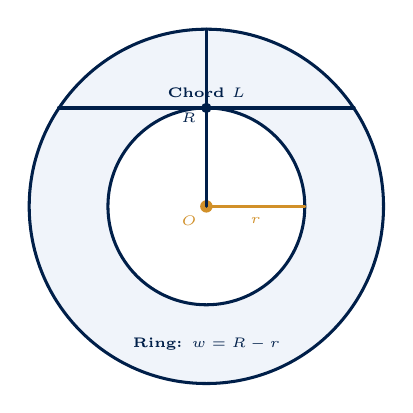
\begin{tikzpicture}[scale=1.25, line cap=round, line join=round]
  \draw[primary, fill=primarylight, line width=1.1pt] (0,0) circle (1.8cm);
  \draw[primary, fill=white, line width=1.1pt] (0,0) circle (1.0cm);

  \fill[accent] (0,0) circle (1.8pt) node[below left, font=\tiny\bfseries]{$O$};
  \draw[accent, line width=1.1pt] (0,0) -- (1.0,0) node[midway, below, font=\tiny\bfseries]{$r$};
  \draw[primary, line width=1.1pt] (0,0) -- (0,1.8) node[midway, left, font=\tiny\bfseries]{$R$};

  \coordinate (T1) at (-1.5,1.0);
  \coordinate (T2) at (1.5,1.0);
  \draw[reddeep, line width=1.2pt] (T1) -- (T2) node[midway, above, font=\tiny\bfseries\color{reddeep}]{Chord $L$};
  \fill[reddeep] (0,1.0) circle (1.5pt);

  \node[font=\tiny\bfseries\color{navy}, align=center] at (0,-1.4) {Ring: $w = R - r$};
\end{tikzpicture}
\end{minipage}\hfill
\begin{minipage}[c]{0.56\textwidth}
\begin{formulaBox}
  \textbf{Master Formulas for Annulus (Outer $R$, Inner $r$):}
  \begin{itemize}
    \item \textbf{Width of Ring ($w$):} $\mathbf{w = R - r}$
    \item \textbf{Area of Ring ($A$):}
      $$\mathbf{A = \pi R^2 - \pi r^2 = \pi(R^2 - r^2) = \pi(R+r)(R-r)}$$
    \item \textbf{In Terms of Ring Width $w$:} $\mathbf{A = \pi w (2r + w)}$
    \item \textbf{Tangent Chord Theorem:} If a chord of outer circle of length $L$ touches inner circle:
      $$\mathbf{A = \frac{\pi L^2}{4}} \quad \left(\text{since } R^2 - r^2 = (L/2)^2\right)$$
  \end{itemize}
\end{formulaBox}
\end{minipage}

\vspace{0.8mm}
\subhead{5.2 The Athletic Running Track Model (Board Classic)}

A standard running track has two parallel straight lines joined by two semicircular ends:

\begin{center}
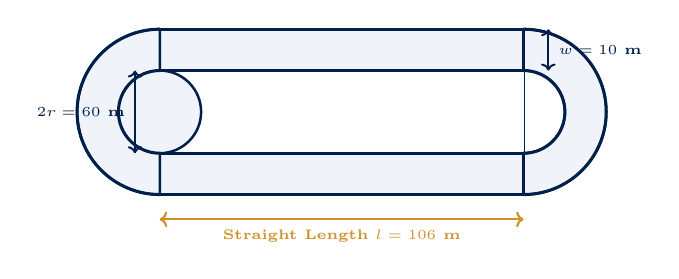
\begin{tikzpicture}[scale=1.05, line cap=round, line join=round]
  \draw[primary, fill=primarylight, line width=0.9pt] (-2.2,-1.0) rectangle (2.2,1.0);
  \fill[white] (-2.2,-0.5) rectangle (2.2,0.5);

  \draw[primary, fill=primarylight, line width=0.9pt] (-2.2,1.0) arc (90:270:1.0cm) -- (-2.2,-0.5) arc (-90:90:0.5cm) -- cycle;
  \draw[primary, fill=primarylight, line width=0.9pt] (2.2,1.0) arc (90:-90:1.0cm) -- (2.2,-0.5) arc (-90:90:0.5cm) -- cycle;

  \draw[primary, line width=1.1pt] (-2.2,1.0) -- (2.2,1.0);
  \draw[primary, line width=1.1pt] (-2.2,-1.0) -- (2.2,-1.0);
  \draw[primary, line width=1.1pt] (-2.2,0.5) -- (2.2,0.5);
  \draw[primary, line width=1.1pt] (-2.2,-0.5) -- (2.2,-0.5);
  \draw[primary, line width=1.1pt] (-2.2,1.0) arc (90:270:1.0cm);
  \draw[primary, line width=1.1pt] (2.2,1.0) arc (90:-90:1.0cm);
  \draw[primary, line width=1.1pt] (-2.2,0.5) arc (90:270:0.5cm);
  \draw[primary, line width=1.1pt] (2.2,0.5) arc (90:-90:0.5cm);

  \draw[{<[scale=0.8]}-{>[scale=0.8]}, accent, line width=0.8pt] (-2.2,-1.3) -- (2.2,-1.3) node[midway, below, font=\tiny\bfseries]{Straight Length $l = 106\text{ m}$};
  \draw[{<[scale=0.8]}-{>[scale=0.8]}, reddeep, line width=0.7pt] (2.5,0.5) -- (2.5,1.0) node[midway, right, font=\tiny\bfseries\color{reddeep}]{$w = 10\text{ m}$};
  \draw[{<[scale=0.8]}-{>[scale=0.8]}, primary, line width=0.7pt] (-2.5,-0.5) -- (-2.5,0.5) node[midway, left, font=\tiny\bfseries]{$2r = 60\text{ m}$};
\end{tikzpicture}
\end{center}

\begin{formulaBox}
  \textbf{Running Track Equations (Straight length $l$, inner radius $r$, outer radius $R = r + w$):}
  \begin{itemize}
    \item \textbf{Inner Perimeter:} $\mathbf{P_{\text{inner}} = 2l + 2\pi r}$
    \item \textbf{Outer Perimeter:} $\mathbf{P_{\text{outer}} = 2l + 2\pi R = 2l + 2\pi(r + w)}$
    \item \textbf{Area of Running Track:}
      $$\mathbf{\text{Area} = 2(l \times w) + \pi(R^2 - r^2) = 2lw + \pi w(2r + w)}$$
  \end{itemize}
\end{formulaBox}

\newpage

% =============================================================================
% PAGE 7: MODULE 6 — INSCRIBED & CIRCUMSCRIBED CIRCLES WITH POLYGONS
% =============================================================================
\thispagestyle{fancy}
\vspace*{0mm}

\chapterbanner{11}{AREAS RELATED TO CIRCLES}{Module 6 $\vert$ Inscribed \& Circumscribed Circles with Polygons}{\CoreTag}

\subhead{6.1 Circle Inscribed in a Square vs Square Inscribed in a Circle}

\begin{center}
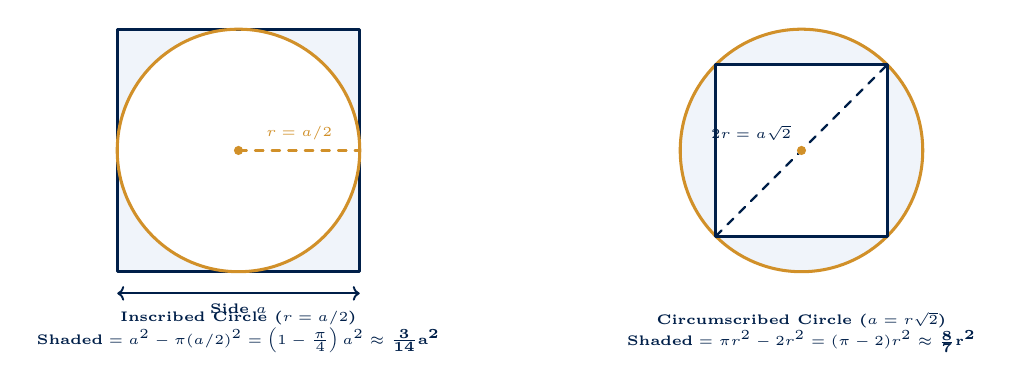
\begin{tikzpicture}[scale=1.1, line cap=round, line join=round]
  % Case A: Circle inside Square
  \begin{scope}[shift={(0,0)}]
    \fill[primarylight] (-1.4,-1.4) rectangle (1.4,1.4);
    \fill[white] (0,0) circle (1.4cm);
    \draw[primary, line width=1.1pt] (-1.4,-1.4) rectangle (1.4,1.4);
    \draw[accent, line width=1.1pt] (0,0) circle (1.4cm);
    \draw[{<[scale=0.8]}-{>[scale=0.8]}, primary, line width=0.7pt] (-1.4,-1.65) -- (1.4,-1.65) node[midway, below, font=\tiny\bfseries]{Side $a$};
    \draw[dashed, accent, line width=0.8pt] (0,0) -- (1.4,0) node[midway, above, font=\tiny\bfseries]{$r = a/2$};
    \fill[accent] (0,0) circle (1.5pt);
    \node[font=\tiny\bfseries\color{navy}, align=center] at (0,-2.1) {\textbf{Inscribed Circle ($r = a/2$)}\\$\text{Shaded} = a^2 - \pi(a/2)^2 = \left(1 - \frac{\pi}{4}\right)a^2 \approx \mathbf{\frac{3}{14}a^2}$};
  \end{scope}

  % Case B: Square inside Circle
  \begin{scope}[shift={(6.5,0)}]
    \fill[primarylight] (0,0) circle (1.4cm);
    \fill[white] (-0.99,-0.99) rectangle (0.99,0.99);
    \draw[accent, line width=1.1pt] (0,0) circle (1.4cm);
    \draw[primary, line width=1.1pt] (-0.99,-0.99) rectangle (0.99,0.99);
    \draw[dashed, reddeep, line width=0.8pt] (-0.99,-0.99) -- (0.99,0.99) node[midway, above left, font=\tiny\bfseries]{$2r = a\sqrt{2}$};
    \fill[accent] (0,0) circle (1.5pt);
    \node[font=\tiny\bfseries\color{navy}, align=center] at (0,-2.1) {\textbf{Circumscribed Circle ($a = r\sqrt{2}$)}\\$\text{Shaded} = \pi r^2 - 2r^2 = (\pi - 2)r^2 \approx \mathbf{\frac{8}{7}r^2}$};
  \end{scope}
\end{tikzpicture}
\end{center}

\vspace{0.8mm}
\begin{formulaBox}
  \textbf{Comparative Ratio Summary for Squares and Circles:}
  \begin{itemize}
    \item \textbf{Inscribed Circle:} $\frac{\text{Area of Circle}}{\text{Area of Square}} = \mathbf{\frac{\pi}{4}} \approx \mathbf{\frac{11}{14}} \approx 78.5\% \implies \text{Shaded Corners} \approx \mathbf{\frac{3}{14}a^2} \approx 21.5\%$.
    \item \textbf{Circumscribed Circle:} $\frac{\text{Area of Square}}{\text{Area of Circle}} = \mathbf{\frac{2}{\pi}} \approx \mathbf{\frac{7}{11}} \approx 63.6\% \implies \text{Shaded Boundary} \approx \mathbf{\frac{4}{11}\pi r^2}$.
  \end{itemize}
\end{formulaBox}

\vspace{0.8mm}
\subhead{6.2 Circles and Equilateral Triangles (Inradius \& Circumradius)}

For an equilateral triangle of side $a$ and height $h = \frac{\sqrt{3}}{2}a$:
\begin{itemize}
  \item \textbf{Inradius ($r$):} $\mathbf{r = \frac{h}{3} = \frac{a}{2\sqrt{3}}} \implies \mathbf{\text{Area of Inscribed Circle} = \pi r^2 = \frac{\pi a^2}{12}}$.
  \item \textbf{Circumradius ($R$):} $\mathbf{R = \frac{2h}{3} = \frac{a}{\sqrt{3}} = 2r} \implies \mathbf{\text{Area of Circumscribed Circle} = \pi R^2 = \frac{\pi a^2}{3} = 4 \times (\text{Incircle Area})}$.
  \item \textbf{Area of Equilateral Triangle:} $\text{Area} = \frac{\sqrt{3}}{4}a^2$.
\end{itemize}

\begin{conceptBox}[title={Worked Archetype 4 $\vert$ Equilateral Triangle \& Circumscribed Circle},fonttitle=\bfseries\color{navy}]
  \textbf{Problem:} A circular table cover of radius $32\text{ cm}$ has an equilateral triangle $ABC$ inscribed inside it. Find the area of the design pattern outside the triangle.
  \par\vspace{0.6mm}\noindent
  \textbf{Step 1: Circle Area:} $R = 32\text{ cm} \implies A_{\text{circle}} = \frac{22}{7} \times 32 \times 32 = \mathbf{\frac{22528}{7}\text{ cm}^2}$.\\
  \textbf{Step 2: Triangle Side $a$:} $R = \frac{a}{\sqrt{3}} \implies a = 32\sqrt{3}\text{ cm}$.\\
  \textbf{Step 3: Triangle Area:} $\text{Area} = \frac{\sqrt{3}}{4}a^2 = \frac{\sqrt{3}}{4}(32\sqrt{3})^2 = \frac{\sqrt{3}}{4}(1024 \times 3) = \mathbf{768\sqrt{3}\text{ cm}^2}$.\\
  \textbf{Step 4: Design Area:} $\mathbf{\text{Design Area}} = \mathbf{\left(\frac{22528}{7} - 768\sqrt{3}\right)\text{ cm}^2}$.
\end{conceptBox}

\newpage

% =============================================================================
% PAGE 8: MODULE 7 — THE TETHERED / GRAZING ANIMAL DYNAMICS
% =============================================================================
\thispagestyle{fancy}
\vspace*{0mm}

\chapterbanner{11}{AREAS RELATED TO CIRCLES}{Module 7 $\vert$ The Tethered / Grazing Animal Dynamics}{\CoreTag}

\subhead{7.1 Physical Intuition: Corner Angle as Sector Angle}

When an animal is tethered by a rope of length $r$ to a peg at a corner of a field:
\begin{enumerate}
  \item The length of the rope acts as the \textbf{radius}: $\mathbf{r = \text{rope length}}$.
  \item The interior corner angle of the field acts as the \textbf{central angle $\theta$}:
    \begin{itemize}
      \item Corner of a \textbf{Square / Rectangle}: $\mathbf{\theta = 90^\circ} \implies \text{Grazing Area} = \mathbf{\frac{1}{4}\pi r^2}$ (Quadrant).
      \item Corner of an \textbf{Equilateral Triangle}: $\mathbf{\theta = 60^\circ} \implies \text{Grazing Area} = \mathbf{\frac{1}{6}\pi r^2}$.
      \item Pegged at \textbf{middle of straight wall}: $\mathbf{\theta = 180^\circ} \implies \text{Grazing Area} = \mathbf{\frac{1}{2}\pi r^2}$ (Semicircle).
      \item Open field (no walls): $\mathbf{\theta = 360^\circ} \implies \text{Grazing Area} = \mathbf{\pi r^2}$ (Full Circle).
    \end{itemize}
\end{enumerate}

\begin{center}
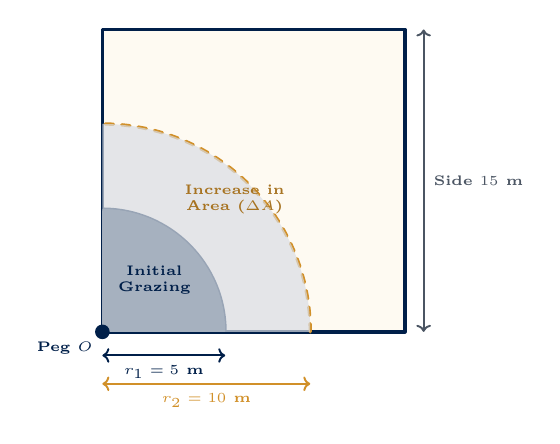
\begin{tikzpicture}[scale=1.2, line cap=round, line join=round]
  \fill[accentlight] (0,0) rectangle (3.2,3.2);
  \draw[primary, line width=1.3pt] (0,0) rectangle (3.2,3.2);

  \fill[primary!35] (0,0) -- (1.3,0) arc (0:90:1.3cm) -- cycle;
  \draw[primary, line width=1.1pt] (1.3,0) arc (0:90:1.3cm);

  \draw[accent, line width=1.2pt, dashed] (2.2,0) arc (0:90:2.2cm);
  \fill[primary!15, opacity=0.7] (0,0) -- (2.2,0) arc (0:90:2.2cm) -- cycle;
  \fill[primary!35] (0,0) -- (1.3,0) arc (0:90:1.3cm) -- cycle;

  \fill[reddeep] (0,0) circle (2.2pt) node[below left, font=\tiny\bfseries\color{reddeep}]{Peg $O$};

  \draw[{<[scale=0.8]}-{>[scale=0.8]}, primary, line width=0.7pt] (0,-0.25) -- (1.3,-0.25) node[midway, below, font=\tiny\bfseries]{$r_1 = 5\text{ m}$};
  \draw[{<[scale=0.8]}-{>[scale=0.8]}, accent, line width=0.7pt] (0,-0.55) -- (2.2,-0.55) node[midway, below, font=\tiny\bfseries]{$r_2 = 10\text{ m}$};
  \draw[{<[scale=0.8]}-{>[scale=0.8]}, secondary, line width=0.7pt] (3.4,0) -- (3.4,3.2) node[midway, right, font=\tiny\bfseries]{Side $15\text{ m}$};

  \node[font=\tiny\bfseries\color{navy}, align=center] at (0.55,0.55) {Initial\\Grazing};
  \node[font=\tiny\bfseries\color{accent!80!black}, align=center] at (1.4,1.4) {Increase in\\Area ($\Delta A$)};
\end{tikzpicture}
\end{center}

\vspace{0.8mm}
\begin{formulaBox}
  \textbf{Increase in Grazing Area When Rope is Extended from $r_1$ to $r_2$:}
  $$\mathbf{\Delta A = \frac{\theta}{360^\circ}\pi \left(r_2^2 - r_1^2\right) = \frac{\theta}{360^\circ}\pi (r_2 + r_1)(r_2 - r_1)}$$
\end{formulaBox}

\begin{conceptBox}[title={Worked Archetype 5 $\vert$ Standard Board Exam Horse Grazing Model},fonttitle=\bfseries\color{navy}]
  \textbf{Problem:} A horse is tied to a peg at one corner of a square grass field of side $15\text{ m}$ by a $5\text{ m}$ long rope. Find: (i) the area in which the horse can graze, and (ii) the increase in grazing area if the rope were $10\text{ m}$ long. (Use $\pi = 3.14$)
  \par\vspace{0.6mm}\noindent
  \textbf{(i) Initial grazing area ($r_1 = 5\text{ m}$, $\theta = 90^\circ$):}
  $$A_1 = \frac{90^\circ}{360^\circ} \times \pi r_1^2 = \frac{1}{4} \times 3.14 \times 25 = \mathbf{19.625\text{ m}^2}$$
  \textbf{(ii) Grazing area with extended rope ($r_2 = 10\text{ m}$):}
  $$A_2 = \frac{1}{4} \times \pi r_2^2 = \frac{1}{4} \times 3.14 \times 100 = 78.5\text{ m}^2$$
  \textbf{Increase in grazing area ($\Delta A$):}
  $$\mathbf{\Delta A} = A_2 - A_1 = 78.5 - 19.625 = \mathbf{58.875\text{ m}^2}$$
\end{conceptBox}

\newpage

% =============================================================================
% PAGE 9: MODULE 8 — QUADRANT & SEMICIRCLE OVERLAPS (THE FAMOUS LEAF/PETAL)
% =============================================================================
\thispagestyle{fancy}
\vspace*{0mm}

\chapterbanner{11}{AREAS RELATED TO CIRCLES}{Module 8 $\vert$ Composite Overlaps: The Famous Petal / Leaf Geometry}{\CoreTag}

\subhead{8.1 The Intersecting Quadrants ``Leaf / Lens'' in a Square}

When two circular quadrants of radius $a$ are drawn inside a square of side $a$ with opposite vertices as centers, they overlap to form a central \textbf{leaf/petal shaped region}:

\begin{minipage}[c]{0.42\textwidth}
\centering
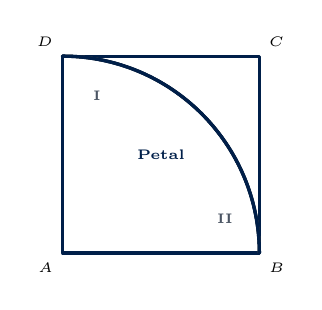
\begin{tikzpicture}[scale=1.25, line cap=round, line join=round]
  \draw[primary, line width=1.1pt] (0,0) rectangle (2.0,2.0);

  \draw[accent, line width=1pt] (2.0,0) arc (0:90:2.0cm);
  \draw[accent, line width=1pt] (0,2.0) arc (90:0:2.0cm);

  \begin{scope}
    \clip (0,0) -- (2.0,0) arc (0:90:2.0cm) -- cycle;
    \fill[primary!40] (2.0,2.0) -- (0,2.0) arc (90:0:2.0cm) -- cycle;
  \end{scope}

  \draw[primary, line width=1.2pt] (2.0,0) arc (0:90:2.0cm);
  \draw[primary, line width=1.2pt] (0,2.0) arc (90:0:2.0cm);

  \node[below left, font=\tiny\bfseries] at (0,0) {$A$};
  \node[below right, font=\tiny\bfseries] at (2.0,0) {$B$};
  \node[above right, font=\tiny\bfseries] at (2.0,2.0) {$C$};
  \node[above left, font=\tiny\bfseries] at (0,2.0) {$D$};

  \node[font=\tiny\bfseries\color{navy}] at (1.0,1.0) {Petal};
  \node[font=\tiny\bfseries\color{secondary}] at (0.35,1.6) {I};
  \node[font=\tiny\bfseries\color{secondary}] at (1.65,0.35) {II};
\end{tikzpicture}
\end{minipage}\hfill
\begin{minipage}[c]{0.56\textwidth}
\begin{formulaBox}
  \textbf{Master Algebraic Derivation of the Petal Area:}
  \begin{enumerate}
    \item $Q_1 + Q_2 = \text{Area of Square} + \text{Area of Petal}$.
    \item $\mathbf{A_{\text{petal}} = 2\left(\frac{1}{4}\pi a^2\right) - a^2 = \left(\frac{\pi}{2} - 1\right)a^2}$.
    \item For $\pi = \frac{22}{7}$:
      $$\mathbf{A_{\text{petal}} = \left(\frac{11}{7} - 1\right)a^2 = \frac{4}{7}a^2}$$
    \item \textbf{Unshaded Corners (I + II):}
      $$\mathbf{A_{\text{unshaded}} = a^2 - \frac{4}{7}a^2 = \frac{3}{7}a^2}$$
  \end{enumerate}
\end{formulaBox}
\end{minipage}

\vspace{0.8mm}
\subhead{8.2 The Four-Petal Flower in a Square (Overlapping Semicircles)}

When four semicircles are drawn on the four sides of a square as diameters, they intersect to create a \textbf{four-petaled symmetrical flower}:

\begin{minipage}[c]{0.42\textwidth}
\centering
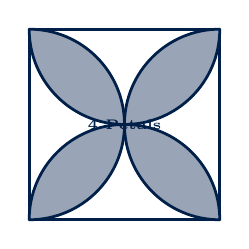
\begin{tikzpicture}[scale=1.1, line cap=round, line join=round]
  \draw[primary, line width=1.1pt] (-1.1,-1.1) rectangle (1.1,1.1);

  \begin{scope}
    \clip (-1.1,-1.1) arc (-90:90:1.1cm) -- cycle;
    \fill[primary!40] (-1.1,-1.1) arc (180:0:1.1cm) -- cycle;
  \end{scope}
  \begin{scope}
    \clip (1.1,1.1) arc (90:270:1.1cm) -- cycle;
    \fill[primary!40] (-1.1,-1.1) arc (180:0:1.1cm) -- cycle;
  \end{scope}
  \begin{scope}
    \clip (-1.1,-1.1) arc (-90:90:1.1cm) -- cycle;
    \fill[primary!40] (1.1,1.1) arc (0:-180:1.1cm) -- cycle;
  \end{scope}
  \begin{scope}
    \clip (1.1,1.1) arc (90:270:1.1cm) -- cycle;
    \fill[primary!40] (1.1,1.1) arc (0:-180:1.1cm) -- cycle;
  \end{scope}

  \draw[primary, line width=1pt] (-1.1,-1.1) arc (-90:90:1.1cm);
  \draw[primary, line width=1pt] (1.1,1.1) arc (90:270:1.1cm);
  \draw[primary, line width=1pt] (-1.1,-1.1) arc (180:0:1.1cm);
  \draw[primary, line width=1pt] (1.1,1.1) arc (0:-180:1.1cm);

  \node[font=\tiny\bfseries\color{navy}] at (0,0) {4 Petals};
\end{tikzpicture}
\end{minipage}\hfill
\begin{minipage}[c]{0.56\textwidth}
\begin{formulaBox}
  \textbf{Four-Petal Flower Equations (Side $a$, $r = a/2$):}
  \begin{itemize}
    \item Total Area of 4 Semicircles:
      $$4 \times \left(\frac{1}{2}\pi r^2\right) = 2\pi (a/2)^2 = \frac{\pi a^2}{2}$$
    \item Total Area of 4 Petals:
      $$\mathbf{A_{\text{4 petals}} = \frac{\pi a^2}{2} - a^2 = \left(\frac{\pi}{2} - 1\right)a^2 = \frac{4}{7}a^2}$$
    \item \textbf{Identity:} The single large leaf and the 4 small petals have the \textbf{exact same area} $\mathbf{\frac{4}{7}a^2}$!
  \end{itemize}
\end{formulaBox}
\end{minipage}

\vspace{0.8mm}
\begin{conceptBox}[title={Worked Archetype 6 $\vert$ Designed Petal Region in a Square},fonttitle=\bfseries\color{navy}]
  \textbf{Problem:} Calculate the area of the designed region common between two quadrants of circles of radius $8\text{ cm}$ each inside a square of side $8\text{ cm}$. (Take $\pi = \frac{22}{7}$)
  \par\vspace{0.6mm}\noindent
  \textbf{Solution:} Here $a = 8\text{ cm}$. Using the direct Maths Manthan Petal Formula:
  $$\text{Area} = \left(\frac{\pi}{2} - 1\right)a^2 = \frac{4}{7}a^2 = \frac{4}{7} \times 8^2 = \frac{256}{7} = \mathbf{36.57\text{ cm}^2}$$
\end{conceptBox}

\newpage

% =============================================================================
% PAGE 10: MODULE 9 — CLOCK HANDS, WIPER BLADES & KINEMATIC SWEEPS
% =============================================================================
\thispagestyle{fancy}
\vspace*{0mm}

\chapterbanner{11}{AREAS RELATED TO CIRCLES}{Module 9 $\vert$ Kinematic Sweeps: Clock Hands \& Wiper Blades}{\CoreTag}

\subhead{9.1 The Angular Velocities of Clock Hands}

A circular clock dial is divided into $12$ hours and $60$ minutes ($360^\circ$ circle):

\begin{minipage}[c]{0.42\textwidth}
\centering
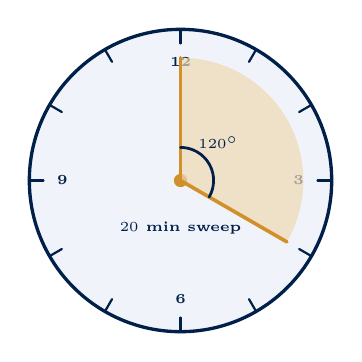
\begin{tikzpicture}[scale=1.2, line cap=round, line join=round]
  \draw[primary, fill=primarylight, line width=1.2pt] (0,0) circle (1.6cm);
  \fill[accent] (0,0) circle (2pt);

  \foreach \a in {0,30,...,330} {
    \draw[primary, line width=0.8pt] (\a:1.45cm) -- (\a:1.6cm);
  }
  \node[font=\tiny\bfseries\color{navy}] at (0,1.25) {12};
  \node[font=\tiny\bfseries\color{navy}] at (1.25,0) {3};
  \node[font=\tiny\bfseries\color{navy}] at (0,-1.25) {6};
  \node[font=\tiny\bfseries\color{navy}] at (-1.25,0) {9};

  \fill[accent!35, opacity=0.7] (0,0) -- (0,1.3) arc (90:-30:1.3cm) -- cycle;
  \draw[accent, line width=1.3pt] (0,0) -- (0,1.3);
  \draw[accent, line width=1.3pt] (0,0) -- ({1.3*cos(-30)},{1.3*sin(-30)});
  \draw[reddeep, line width=1pt] (0,0.35) arc (90:-30:0.35cm);
  \node[font=\tiny\bfseries\color{reddeep}] at (0.4,0.4) {$120^\circ$};

  \node[font=\tiny\bfseries\color{navy}, align=center] at (0,-0.5) {$20\text{ min sweep}$};
\end{tikzpicture}
\end{minipage}\hfill
\begin{minipage}[c]{0.56\textwidth}
\begin{formulaBox}
  \textbf{Angular Velocities of Clock Hands:}
  \begin{itemize}
    \item \textbf{Minute Hand:}
      $$\text{Speed} = \frac{360^\circ}{60\text{ min}} = \mathbf{6^\circ/\text{minute}}$$
      $$\mathbf{\text{Angle in } m \text{ minutes: } \theta = 6m^\circ}$$
    \item \textbf{Hour Hand:}
      $$\text{Speed} = \frac{360^\circ}{720\text{ min}} = \mathbf{0.5^\circ/\text{minute} = \left(\frac{1}{2}\right)^\circ/\text{min}}$$
      $$\mathbf{\text{In 1 hour (60 min): } \theta = 30^\circ}$$
  \end{itemize}
\end{formulaBox}
\end{minipage}

\vspace{0.8mm}
\subhead{9.2 Automobile Windshield Wipers (Twin Sweeps)}

\begin{formulaBox}
  $$\mathbf{\text{Total Area Cleaned at Each Sweep}} = \mathbf{2 \times \left(\frac{\theta}{360^\circ} \times \pi r^2\right)}$$
\end{formulaBox}

\vspace{0.8mm}
\begin{conceptBox}[title={Worked Archetype 7 $\vert$ Minute Hand Swept Area},fonttitle=\bfseries\color{navy}]
  \textbf{Problem:} The length of the minute hand of a clock is $14\text{ cm}$. Find the area swept by the minute hand in $5\text{ minutes}$. (Take $\pi = \frac{22}{7}$)
  \par\vspace{0.6mm}\noindent
  \textbf{Step 1: Angle swept:} $\theta = 5\text{ min} \times 6^\circ/\text{min} = 30^\circ$.\\
  \textbf{Step 2: Area swept:} $\text{Area} = \frac{30^\circ}{360^\circ} \times \frac{22}{7} \times 14^2 = \frac{1}{12} \times 22 \times 2 \times 14 = \mathbf{\frac{154}{3}\text{ cm}^2 \approx 51.33\text{ cm}^2}$.
\end{conceptBox}

\vspace{0.8mm}
\begin{conceptBox}[title={Worked Archetype 8 $\vert$ Car Windshield Twin Wipers},fonttitle=\bfseries\color{navy}]
  \textbf{Problem:} A car has two non-overlapping wipers with blade length $25\text{ cm}$ sweeping angle $115^\circ$. Find total cleaned area per sweep. (Take $\pi = \frac{22}{7}$)
  \par\vspace{0.6mm}\noindent
  $$\text{Total Area} = 2 \times \left(\frac{115^\circ}{360^\circ} \times \frac{22}{7} \times 25^2\right) = 2 \times \frac{23}{72} \times \frac{22}{7} \times 625 = \mathbf{\frac{158125}{126}\text{ cm}^2 \approx 1254.96\text{ cm}^2}$$
\end{conceptBox}

\newpage

% =============================================================================
% PAGE 11: MODULE 10 — ADVANCED COMBINATIONS: BROOCHES & HIPPOCRATES LUNULAE
% =============================================================================
\thispagestyle{fancy}
\vspace*{0mm}

\chapterbanner{11}{AREAS RELATED TO CIRCLES}{Module 10 $\vert$ Advanced Combinations: Brooches \& Hippocrates Lunulae}{\CoreTag}

\subhead{10.1 The Circular Brooch with Silver Wire Diameters}

A popular board exam configuration involves a decorative circular brooch crafted with silver wire:

\begin{minipage}[c]{0.42\textwidth}
\centering
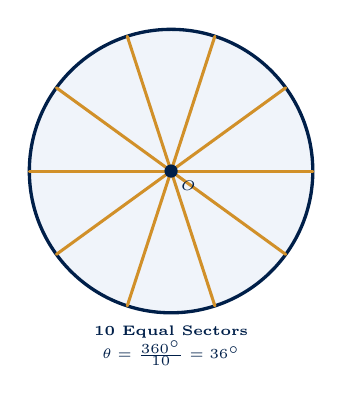
\begin{tikzpicture}[scale=1.2, line cap=round, line join=round]
  \draw[primary, fill=primarylight, line width=1.2pt] (0,0) circle (1.5cm);

  \foreach \i in {0,1,2,3,4} {
    \draw[accent, line width=1.1pt] ({\i*36}:1.5cm) -- ({180 + \i*36}:1.5cm);
  }
  \fill[reddeep] (0,0) circle (2pt) node[below right, font=\tiny\bfseries\color{reddeep}]{$O$};

  \node[font=\tiny\bfseries\color{navy}, align=center] at (0,-1.85) {10 Equal Sectors\\$\theta = \frac{360^\circ}{10} = 36^\circ$};
\end{tikzpicture}
\end{minipage}\hfill
\begin{minipage}[c]{0.56\textwidth}
\begin{formulaBox}
  \textbf{Equations for Brooch of Diameter $d$ with $k$ Diameters:}
  \begin{itemize}
    \item \textbf{Total Length of Silver Wire ($L$):}
      $$\mathbf{L = \pi d + k \cdot d = d(\pi + k)}$$
      For standard board problem ($k = 5$ diameters):
      $$\mathbf{L = \pi d + 5d = d\left(\frac{22}{7} + 5\right) = \frac{57}{7}d}$$
    \item \textbf{Central Angle of Each Sector:} $\mathbf{\theta = \frac{360^\circ}{2k} = 36^\circ}$
    \item \textbf{Area of Each Sector:} $\mathbf{A = \frac{1}{10}\pi r^2 = \frac{\pi d^2}{40}}$
  \end{itemize}
\end{formulaBox}
\end{minipage}

\vspace{0.8mm}
\subhead{10.2 Hippocrates Lunulae (The Crescent Moon Quadrature Theorem)}

Curved areas can equal rectilinear areas:

\begin{minipage}[c]{0.42\textwidth}
\centering
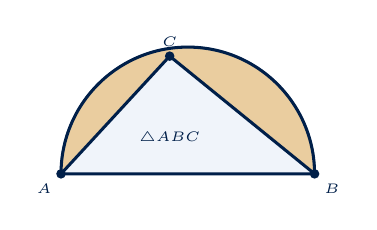
\begin{tikzpicture}[scale=1.15, line cap=round, line join=round]
  \coordinate (A) at (-1.4,0);
  \coordinate (B) at (1.4,0);
  \coordinate (C) at (-0.2,1.3);

  \draw[primary!40, line width=0.9pt] (1.4,0) arc (0:180:1.4cm);
  \fill[accent!45] (A) arc (180:0:1.4cm) -- cycle;
  \fill[primarylight] (A) -- (B) -- (C) -- cycle;

  \draw[primary, line width=1.1pt] (A) -- (B) -- (C) -- cycle;
  \draw[reddeep, line width=1.1pt] (A) arc (180:0:1.4cm);

  \fill[primary] (A) circle (1.5pt) node[below left, font=\tiny]{$A$};
  \fill[primary] (B) circle (1.5pt) node[below right, font=\tiny]{$B$};
  \fill[primary] (C) circle (1.5pt) node[above, font=\tiny]{$C$};

  \node[font=\tiny\bfseries\color{navy}] at (-0.2,0.4) {$\triangle ABC$};
\end{tikzpicture}
\end{minipage}\hfill
\begin{minipage}[c]{0.56\textwidth}
\begin{formulaBox}
  \textbf{Theorem of Hippocrates (Sum of Lunulae):}
  In a right-angled triangle $\triangle ABC$ ($\angle C = 90^\circ$):
  \begin{enumerate}
    \item Semicircles are drawn on legs $a, b$ and hypotenuse $c$.
    \item \textbf{Theorem:} The sum of the areas of the two shaded crescents (lunulae) equals the area of $\triangle ABC$!
      $$\mathbf{\text{Area}(\text{Lune}_1) + \text{Area}(\text{Lune}_2) = \text{Area}(\triangle ABC) = \frac{1}{2}ab}$$
  \end{enumerate}
\end{formulaBox}
\end{minipage}

\vspace{0.8mm}
\begin{conceptBox}[title={Worked Archetype 9 $\vert$ Brooch Silver Wire \& Sector Calculation},fonttitle=\bfseries\color{navy}]
  \textbf{Problem:} A brooch is made with silver wire as a circle with diameter $35\text{ mm}$ and $5$ diameters dividing it into $10$ equal sectors. Find: (i) wire length, and (ii) area of each sector.
  \par\vspace{0.6mm}\noindent
  \textbf{(i) Total Wire Length ($L$):} $L = \pi d + 5d = \left(\frac{22}{7} \times 35\right) + (5 \times 35) = 110 + 175 = \mathbf{285\text{ mm}}$.\\
  \textbf{(ii) Area of each sector ($A$):} $A = \frac{1}{10}\pi r^2 = \frac{1}{10} \times \frac{22}{7} \times \frac{35}{2} \times \frac{35}{2} = \mathbf{\frac{385}{4}\text{ mm}^2 = 96.25\text{ mm}^2}$.
\end{conceptBox}

\newpage

% =============================================================================
% PAGE 12: MODULE 11 — MASTER FORMULA MATRIX & DECISION TREE
% =============================================================================
\thispagestyle{fancy}
\vspace*{0mm}

\chapterbanner{11}{AREAS RELATED TO CIRCLES}{Module 11 $\vert$ Master Formula Matrix \& Decision Protocol}{\ReferenceTag}

\subhead{11.1 The Comprehensive Mensuration Matrix for Circular Geometries}

\begin{center}
\small
\begin{tabularx}{\textwidth}{>{\bfseries}p{28mm} c p{40mm} X}
\toprule
\rowcolor{bluepale}
\textbf{Geometric Figure} & \textbf{Parameters} & \textbf{Boundary / Perimeter ($P$)} & \textbf{Enclosed Surface Area ($A$)} \\
\midrule
\textbf{Full Circle} & $r, d=2r$ & $C = 2\pi r = \pi d$ & $A = \pi r^2 = \frac{1}{4}\pi d^2$ \\
\rowcolor{lightgray}
\textbf{Semicircle} & $r$ & $P = \pi r + 2r = r(\pi + 2)$ & $A = \frac{1}{2}\pi r^2$ \\
\textbf{Quadrant} & $r$ & $P = \frac{1}{2}\pi r + 2r = r\left(\frac{\pi}{2} + 2\right)$ & $A = \frac{1}{4}\pi r^2$ \\
\rowcolor{lightgray}
\textbf{Circular Sector} & $r, \theta$ & $P = \frac{\theta}{360^\circ}(2\pi r) + 2r$ & $A = \frac{\theta}{360^\circ}\pi r^2 = \frac{1}{2}lr$ \\
\textbf{Minor Segment} & $r, \theta$ & $P = \text{Arc } l + 2r\sin(\frac{\theta}{2})$ & $A = \frac{\theta}{360^\circ}\pi r^2 - \frac{1}{2}r^2\sin\theta$ \\
\rowcolor{lightgray}
\textbf{Major Segment} & $r, \theta$ & $P = (2\pi r - l) + 2r\sin(\frac{\theta}{2})$ & $A = \pi r^2 - A_{\text{minor segment}}$ \\
\textbf{Circular Ring (Annulus)} & $R, r$ & $P_{\text{total}} = 2\pi(R + r)$ & $A = \pi(R^2 - r^2) = \pi(R+r)(R-r)$ \\
\rowcolor{lightgray}
\textbf{Square Leaf / Petal} & $a$ & $P = 2 \times \left(\frac{1}{2}\pi a\right) = \pi a$ & $A = \left(\frac{\pi}{2} - 1\right)a^2 \approx \frac{4}{7}a^2$ \\
\bottomrule
\end{tabularx}
\end{center}

\vspace{0.8mm}
\subhead{11.2 The 3-Step Board Examination Decision Flowchart}

\begin{center}
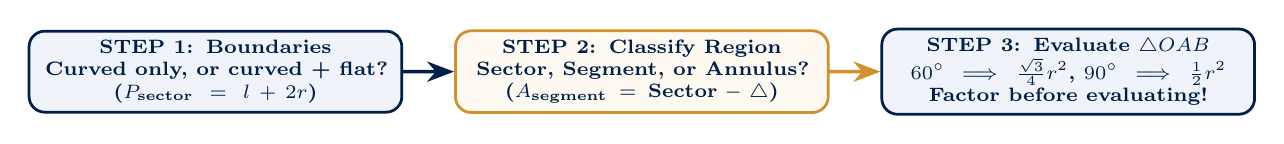
\begin{tikzpicture}[scale=0.95, line cap=round, line join=round]
  \node[draw=primary, fill=primarylight, rounded corners=2mm, line width=1pt, font=\scriptsize\bfseries\color{navy}, align=center, text width=4.5cm] (Q1) at (0,2.5) {STEP 1: Boundaries\\Curved only, or curved + flat?\\($P_{\text{sector}} = l + 2r$)};

  \node[draw=accent, fill=accentlight, rounded corners=2mm, line width=1pt, font=\scriptsize\bfseries\color{navy}, align=center, text width=4.5cm] (Q2) at (5.7,2.5) {STEP 2: Classify Region\\Sector, Segment, or Annulus?\\($A_{\text{segment}} = \text{Sector} - \triangle$)};

  \node[draw=primary, fill=primarylight, rounded corners=2mm, line width=1pt, font=\scriptsize\bfseries\color{navy}, align=center, text width=4.5cm] (Q3) at (11.4,2.5) {STEP 3: Evaluate $\triangle OAB$\\$60^\circ \implies \frac{\sqrt{3}}{4}r^2$, $90^\circ \implies \frac{1}{2}r^2$\\Factor before evaluating!};

  \draw[-{Stealth[scale=1.1]}, primary, line width=1.3pt] (Q1) -- (Q2);
  \draw[-{Stealth[scale=1.1]}, accent, line width=1.3pt] (Q2) -- (Q3);
\end{tikzpicture}
\end{center}

\vspace{0.8mm}
\begin{formulaBox}
  \textbf{Fast Arithmetic Factoring Constants (When $\pi = \frac{22}{7}$):}
  \begin{itemize}
    \item \textbf{Quadrant Perimeter:} $P = \frac{1}{2}\pi r + 2r = \left(\frac{11}{7} + 2\right)r = \mathbf{\frac{25}{7}r}$
    \item \textbf{Semicircle Perimeter:} $P = \pi r + 2r = \left(\frac{22}{7} + 2\right)r = \mathbf{\frac{36}{7}r}$
    \item \textbf{Shaded Corners of Square ($a = 2r$):} $\text{Area} = 4r^2 - \pi r^2 = \left(4 - \frac{22}{7}\right)r^2 = \mathbf{\frac{6}{7}r^2} = \mathbf{\frac{3}{14}a^2}$
    \item \textbf{Single Petal in Square:} $\text{Area} = \left(\frac{\pi}{2} - 1\right)a^2 = \left(\frac{11}{7} - 1\right)a^2 = \mathbf{\frac{4}{7}a^2}$
  \end{itemize}
\end{formulaBox}

\newpage

% =============================================================================
% PAGE 13: MODULE 12 — BOARD EXAM CASE-STUDY & APPLIED MODELING
% =============================================================================
\thispagestyle{fancy}
\vspace*{0mm}

\chapterbanner{11}{AREAS RELATED TO CIRCLES}{Module 12 $\vert$ Board Exam Case-Study \& Applied Modeling}{\ExamTag}

\subhead{Case Study 1 $\vert$ Navigation Marine Lighthouse Warning Sector}

To warn ships of underwater rocks, a coastal lighthouse spreads a red colored light over a sector of angle $80^\circ$ to a distance of $16.5\text{ km}$.

\begin{minipage}[c]{0.40\textwidth}
\centering
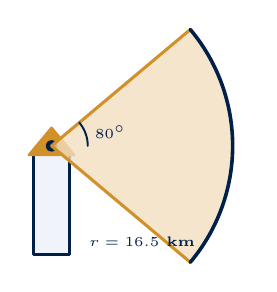
\begin{tikzpicture}[scale=1.15, line cap=round, line join=round]
  \draw[primary, fill=primarylight, line width=1pt] (-0.2,0) rectangle (0.2,1.1);
  \draw[accent, fill=accent, line width=0.9pt] (-0.25,1.1) -- (0.25,1.1) -- (0,1.4) -- cycle;
  \fill[reddeep] (0,1.2) circle (1.8pt);

  \fill[accent!30, opacity=0.8] (0,1.2) -- ({2.0*cos(-40)},{1.2 + 2.0*sin(-40)}) arc (-40:40:2.0cm) -- cycle;
  \draw[accent, line width=1.1pt] (0,1.2) -- ({2.0*cos(-40)},{1.2 + 2.0*sin(-40)});
  \draw[accent, line width=1.1pt] (0,1.2) -- ({2.0*cos(40)},{1.2 + 2.0*sin(40)});
  \draw[reddeep, line width=1.3pt] ({2.0*cos(-40)},{1.2 + 2.0*sin(-40)}) arc (-40:40:2.0cm);

  \draw[reddeep, line width=0.7pt] (0.4,1.2) arc (0:40:0.4cm);
  \node[font=\tiny\bfseries\color{reddeep}] at (0.65,1.35) {$80^\circ$};
  \node[font=\tiny\bfseries\color{navy}, below] at (1.0,0.3) {$r = 16.5\text{ km}$};
\end{tikzpicture}
\end{minipage}\hfill
\begin{minipage}[c]{0.58\textwidth}
\begin{conceptBox}[title={4-Mark Board Question Protocol},fonttitle=\bfseries\color{navy}]
  \textbf{Questions:}
  \begin{enumerate}
    \item What geometric figure represents the illuminated sea surface? [1M]
    \item Calculate the length of the outer warning arc on the ocean. [1M]
    \item Find the area of the sea over which ships are warned. ($\pi = 3.14$) [2M]
  \end{enumerate}
\end{conceptBox}
\end{minipage}

\vspace{0.8mm}
\begin{successBox}[title={Solution \& Marking Scheme Evaluation},fonttitle=\bfseries\color{navy}]
  \begin{enumerate}
    \item \textbf{Geometric Classification [1M]:} The illuminated region is a \textbf{sector of a circle} with radius $r = 16.5\text{ km}$ and central angle $\theta = 80^\circ$.
    \item \textbf{Length of Warning Arc [1M]:}
      $l = \frac{80^\circ}{360^\circ} \times 2 \times 3.14 \times 16.5 = \frac{2}{9} \times 103.62 = \mathbf{23.03\text{ km}}$.
    \item \textbf{Total Area of Sea Warned [2M]:}
      $A = \frac{80^\circ}{360^\circ} \times 3.14 \times (16.5)^2 = \frac{2}{9} \times 3.14 \times 272.25 = \mathbf{189.97\text{ km}^2}$.
  \end{enumerate}
\end{successBox}

\vspace{0.8mm}
\subhead{Case Study 2 $\vert$ Architectural Roundabout with Floral Sectors}

A city municipal corporation designs a circular traffic roundabout of radius $28\text{ m}$. At the center is a circular fountain of radius $7\text{ m}$. The remaining annular region is divided into $6$ congruent sectors: $3$ sectors planted with red roses, and $3$ alternating sectors with green grass.

\begin{conceptBox}[title={Case Study Questions \& Structured Solutions},fonttitle=\bfseries\color{navy}]
  \begin{enumerate}
    \item \textbf{Find the central angle of each sector:} $\theta = \frac{360^\circ}{6} = \mathbf{60^\circ}$.
    \item \textbf{Find the area of the central fountain:} $A_{\text{fountain}} = \pi r^2 = \frac{22}{7} \times 7^2 = \mathbf{154\text{ m}^2}$.
    \item \textbf{Find the total area planted with red roses:}
      $$\text{Total Annular Area} = \pi(R^2 - r^2) = \frac{22}{7}(28^2 - 7^2) = \frac{22}{7}(784 - 49) = \frac{22}{7} \times 735 = 2310\text{ m}^2$$
      Since roses occupy $3$ out of $6$ equal sectors: $\mathbf{\text{Area of Roses}} = \frac{1}{2} \times 2310 = \mathbf{1155\text{ m}^2}$.
  \end{enumerate}
\end{conceptBox}

\newpage

% =============================================================================
% PAGE 14: MODULE 13 — BOARD EXAM TRAPS, HACKS & PRE-SUBMISSION AUDIT
% =============================================================================
\thispagestyle{fancy}
\vspace*{0mm}

\chapterbanner{11}{AREAS RELATED TO CIRCLES}{Module 13 $\vert$ Board Traps, Verification Hacks \& 5-Point Audit}{\ExamTag}

\subhead{13.1 The Top 7 Board Examination Blunders (And How to Neutralize Them)}

\begin{enumerate}[label=\textbf{Trap \arabic*:}, leftmargin=5mm, itemsep=1pt, topsep=0.8pt, parsep=0pt]
  \item \textbf{The Sector Perimeter Omission:} Writing $P = \frac{\theta}{360^\circ}(2\pi r)$ and forgetting to add the two radii. \TrapTag\ Always write $\mathbf{P = l + 2r}$ before substituting numbers!
  \item \textbf{Diameter Substituted as Radius:} When given ``diameter $14\text{ cm}$'', blindly writing $r = 14$. Always write $\mathbf{r = d/2 = 7\text{ cm}}$ in the first line of your solution.
  \item \textbf{Wrong $\pi$ Value Substituted:} Using $\frac{22}{7}$ when instructed ``(Use $\pi = 3.14$)''. This incurs a direct deduction under CBSE marking schemes!
  \item \textbf{Segment Addition Blunder:} Adding the triangle to the sector instead of subtracting: $\text{Segment} = \text{Sector} - \triangle OAB$.
  \item \textbf{Equilateral vs Obtuse Triangle Confusion:} Using $\frac{1}{2}r^2$ for $\theta = 60^\circ$ instead of $\mathbf{\frac{\sqrt{3}}{4}r^2}$.
  \item \textbf{Clock Angle Calculation Error:} Assuming the minute hand moves $1^\circ$ per minute. It moves $\mathbf{6^\circ/\text{minute}}$! The hour hand moves $\mathbf{0.5^\circ/\text{minute}}$.
  \item \textbf{Mixed Linear Units:} Calculating area using radius in centimeters and length in meters. Convert all dimensions to the same unit ($\text{cm}$ or $\text{m}$) before calculating!
\end{enumerate}

\subhead{13.2 High-Speed Algebraic Factorization Protocol}

\begin{tabularx}{\textwidth}{X | X}
\toprule
\rowcolor{redpale}
\textbf{The Slow Method (High Arithmetic Risk)} & \textbf{The Maths Manthan Factoring Method} \\
\midrule
Find annulus area ($R = 14, r = 7$): & Factor algebraic terms first: \\
$\text{Area} = \frac{22}{7} \times 14^2 - \frac{22}{7} \times 7^2$ & $\text{Area} = \pi(R^2 - r^2) = \mathbf{\pi(R+r)(R-r)}$ \\
$= \frac{22}{7} \times 196 - \frac{22}{7} \times 49$ & Substitute once at the end: \\
$= 616 - 154 = \mathbf{462\text{ cm}^2}$ & $= \frac{22}{7} \times (14 + 7) \times (14 - 7) = \frac{22}{7} \times 21 \times 7 = \mathbf{462\text{ cm}^2}$ \\
\bottomrule
\end{tabularx}

\vspace{1mm}
\subhead{13.3 The 5-Point Board Examination Pre-Submission Checklist}

\begin{successBox}[top=1.2mm,bottom=1.2mm,before skip=1.5pt,after skip=1pt]
  \textbf{Final 60-Second Answer Sheet Verification Protocol:}
  \begin{itemize}[leftmargin=4mm,itemsep=1pt,topsep=1pt,parsep=0pt]
    \item[$\square$] \textbf{Dimension Check:} Did you state $r = d/2$ explicitly with correct unified units ($\text{cm}$ or $\text{m}$)?
    \item[$\square$] \textbf{Symbolic Formula Stated:} Did you write the algebraic formula before substituting numbers? (Guarantees CBSE method marks).
    \item[$\square$] \textbf{Specified $\pi$ Respected:} Did you check whether $\pi = \frac{22}{7}$ or $\pi = 3.14$ was requested?
    \item[$\square$] \textbf{Perimeter vs Arc Length:} If asked for perimeter of a sector, did you remember to add $+2r$?
    \item[$\square$] \textbf{Dimensional Units Attached:} Lengths in $\mathbf{\text{cm} / \text{m}}$, Areas in $\mathbf{\text{cm}^2 / \text{m}^2}$, Angles in $\mathbf{^\circ}$!
  \end{itemize}
\end{successBox}

\vfill
\begin{center}
  {\footnotesize\bfseries\color{primary}MATHS MANTHAN TUITION CLASSES \quad$\vert$\quad END OF CHAPTER 11 HANDBOOK}\\[1mm]
  {\scriptsize\color{secondary}Designed for Academic Excellence in CBSE Class 10 Board Examinations 2026--27.}
\end{center}

\end{document}
